\documentclass[14pt]{extbook}
\usepackage{multicol, enumerate, enumitem, hyperref, color, soul, setspace, parskip, fancyhdr} %General Packages
\usepackage{amssymb, amsthm, amsmath, latexsym, units, mathtools} %Math Packages
\everymath{\displaystyle} %All math in Display Style
% Packages with additional options
\usepackage[headsep=0.5cm,headheight=12pt, left=1 in,right= 1 in,top= 1 in,bottom= 1 in]{geometry}
\usepackage[usenames,dvipsnames]{xcolor}
\usepackage{dashrule}  % Package to use the command below to create lines between items
\newcommand{\litem}[1]{\item#1\hspace*{-1cm}\rule{\textwidth}{0.4pt}}
\pagestyle{fancy}
\lhead{Progress Quiz 3}
\chead{}
\rhead{Version C}
\lfoot{3012-8528}
\cfoot{}
\rfoot{Summer C 2021}
\begin{document}

\begin{enumerate}
\litem{
Choose the equation of the function graphed below.
\begin{center}
    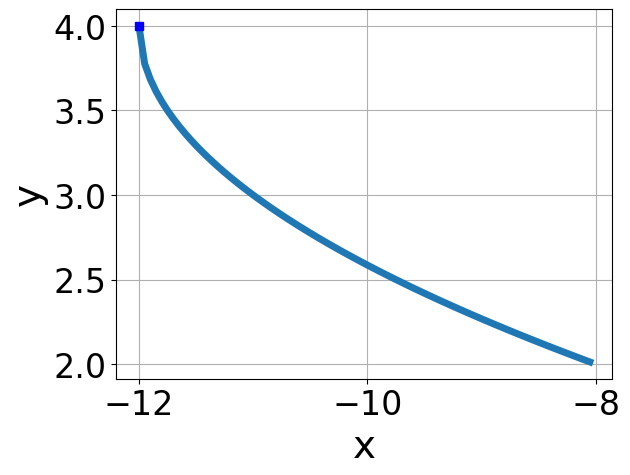
\includegraphics[width=0.5\textwidth]{../Figures/radicalGraphToEquationC.png}
\end{center}
\begin{enumerate}[label=\Alph*.]
\item \( f(x) = - \sqrt[3]{x - 12} + 4 \)
\item \( f(x) = \sqrt[3]{x - 12} + 4 \)
\item \( f(x) = \sqrt[3]{x + 12} + 4 \)
\item \( f(x) = - \sqrt[3]{x + 12} + 4 \)
\item \( \text{None of the above} \)

\end{enumerate} }
\litem{
What is the domain of the function below?\[ f(x) = \sqrt[8]{7 x + 5} \]\begin{enumerate}[label=\Alph*.]
\item \( (-\infty, \infty) \)
\item \( [a, \infty), \text{where } a \in [-1.88, -1.02] \)
\item \( [a, \infty), \text{ where } a \in [-0.82, -0.36] \)
\item \( (-\infty, a], \text{where } a \in [-2.1, -0.83] \)
\item \( (-\infty, a], \text{where } a \in [-0.95, 0.49] \)

\end{enumerate} }
\litem{
Solve the radical equation below. Then, choose the interval(s) that the solution(s) belongs to.\[ \sqrt{9 x - 7} - \sqrt{2 x - 5} = 0 \]\begin{enumerate}[label=\Alph*.]
\item \( x \in [-0.19,0.29] \)
\item \( \text{All solutions lead to invalid or complex values in the equation.} \)
\item \( x \in [1.42,1.95] \)
\item \( x_1 \in [0.42, 1.49] \text{ and } x_2 \in [2.01,2.77] \)
\item \( x_1 \in [-0.19, 0.29] \text{ and } x_2 \in [0.03,0.82] \)

\end{enumerate} }
\litem{
Solve the radical equation below. Then, choose the interval(s) that the solution(s) belongs to.\[ \sqrt{4 x + 6} - \sqrt{6 x + 8} = 0 \]\begin{enumerate}[label=\Alph*.]
\item \( \text{All solutions lead to invalid or complex values in the equation.} \)
\item \( x_1 \in [-2.85, -1.21] \text{ and } x_2 \in [-1.2,-0.66] \)
\item \( x \in [6.06,7.44] \)
\item \( x_1 \in [-2.85, -1.21] \text{ and } x_2 \in [-1.75,-1.28] \)
\item \( x \in [-1.13,-0.94] \)

\end{enumerate} }
\litem{
Choose the equation of the function graphed below.
\begin{center}
    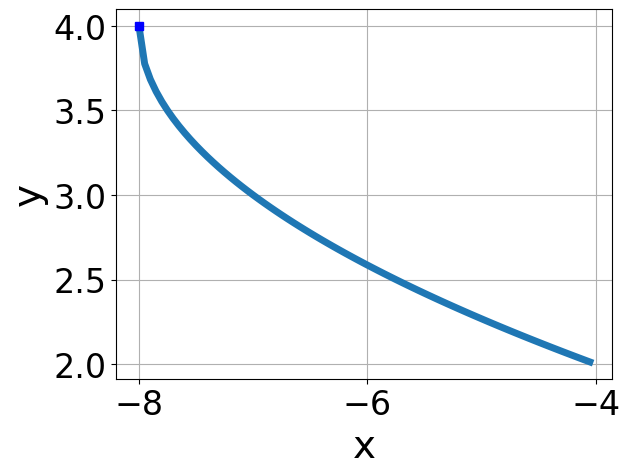
\includegraphics[width=0.5\textwidth]{../Figures/radicalGraphToEquationCopyC.png}
\end{center}
\begin{enumerate}[label=\Alph*.]
\item \( f(x) = \sqrt{x + 8} + 4 \)
\item \( f(x) = - \sqrt{x + 8} + 4 \)
\item \( f(x) = \sqrt{x - 8} + 4 \)
\item \( f(x) = - \sqrt{x - 8} + 4 \)
\item \( \text{None of the above} \)

\end{enumerate} }
\litem{
Solve the radical equation below. Then, choose the interval(s) that the solution(s) belongs to.\[ \sqrt{8 x^2 - 56} - \sqrt{18 x} = 0 \]\begin{enumerate}[label=\Alph*.]
\item \( x \in [-3,-1.6] \)
\item \( \text{All solutions lead to invalid or complex values in the equation.} \)
\item \( x_1 \in [0.8, 2.8] \text{ and } x_2 \in [2,9] \)
\item \( x_1 \in [-3, -1.6] \text{ and } x_2 \in [2,9] \)
\item \( x \in [2.6,4.7] \)

\end{enumerate} }
\litem{
Choose the graph of the equation below.\[ f(x) = - \sqrt{x - 10} + 5 \]\begin{enumerate}[label=\Alph*.]
\begin{multicols}{2}\item 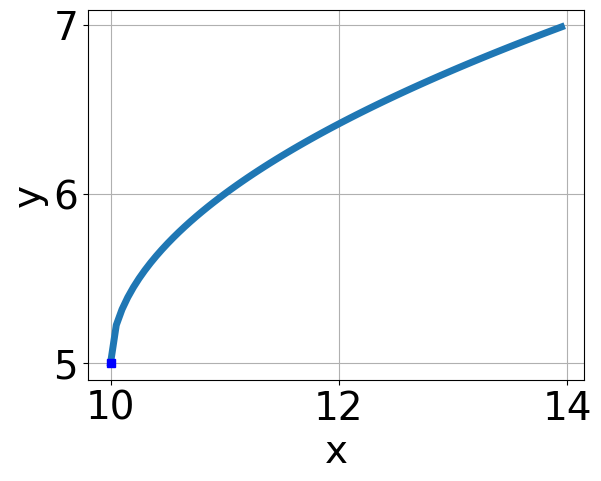
\includegraphics[width = 0.3\textwidth]{../Figures/radicalEquationToGraphAC.png}\item 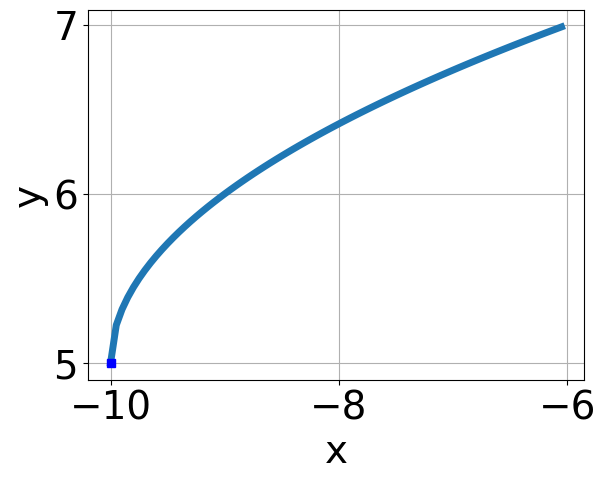
\includegraphics[width = 0.3\textwidth]{../Figures/radicalEquationToGraphBC.png}\item 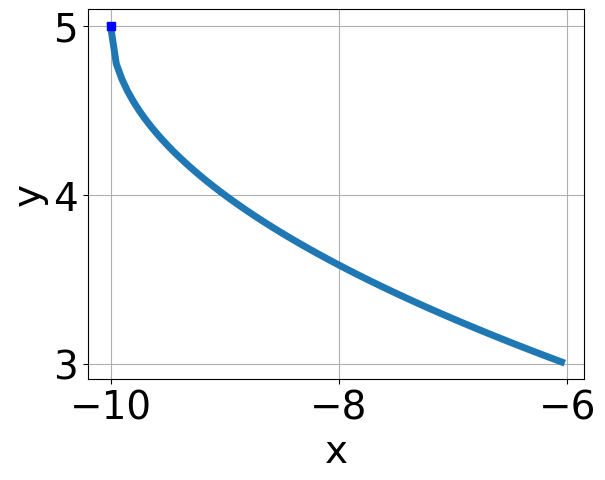
\includegraphics[width = 0.3\textwidth]{../Figures/radicalEquationToGraphCC.png}\item 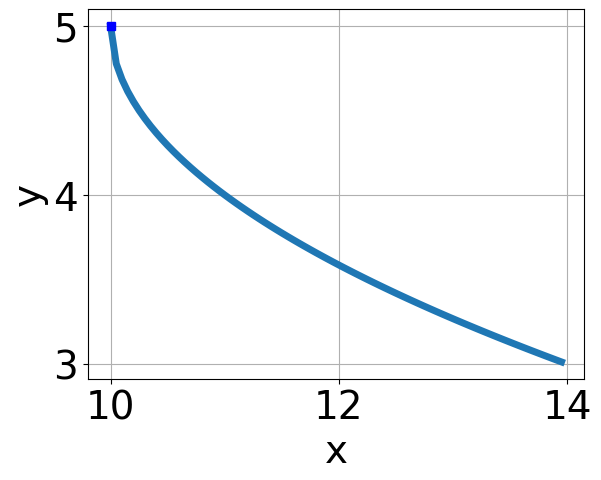
\includegraphics[width = 0.3\textwidth]{../Figures/radicalEquationToGraphDC.png}\end{multicols}\item None of the above.
\end{enumerate} }
\litem{
Solve the radical equation below. Then, choose the interval(s) that the solution(s) belongs to.\[ \sqrt{-56 x^2 - 35} - \sqrt{91 x} = 0 \]\begin{enumerate}[label=\Alph*.]
\item \( x \in [-1.03,-0.83] \)
\item \( x_1 \in [-1.03, -0.83] \text{ and } x_2 \in [-1.25,0.13] \)
\item \( \text{All solutions lead to invalid or complex values in the equation.} \)
\item \( x \in [-0.66,-0.32] \)
\item \( x_1 \in [0.94, 1.32] \text{ and } x_2 \in [0.06,1.18] \)

\end{enumerate} }
\litem{
Choose the graph of the equation below.\[ f(x) = \sqrt{x + 12} + 6 \]\begin{enumerate}[label=\Alph*.]
\begin{multicols}{2}\item 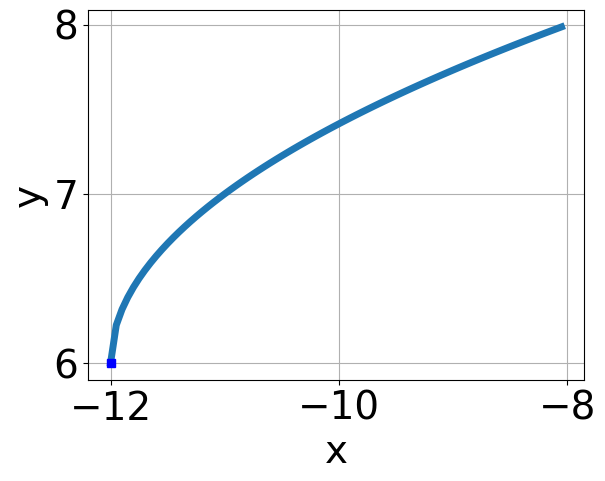
\includegraphics[width = 0.3\textwidth]{../Figures/radicalEquationToGraphCopyAC.png}\item 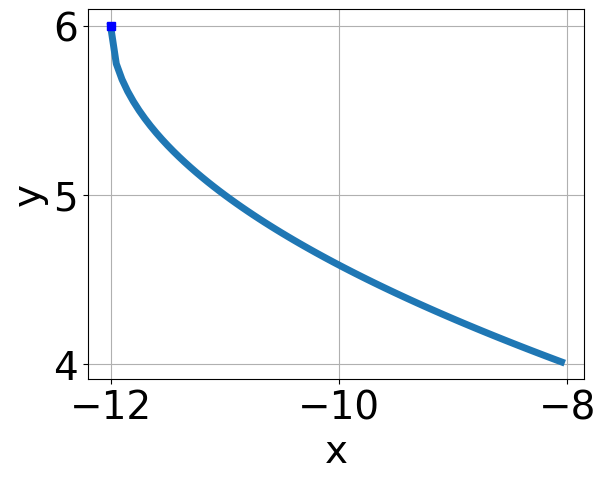
\includegraphics[width = 0.3\textwidth]{../Figures/radicalEquationToGraphCopyBC.png}\item 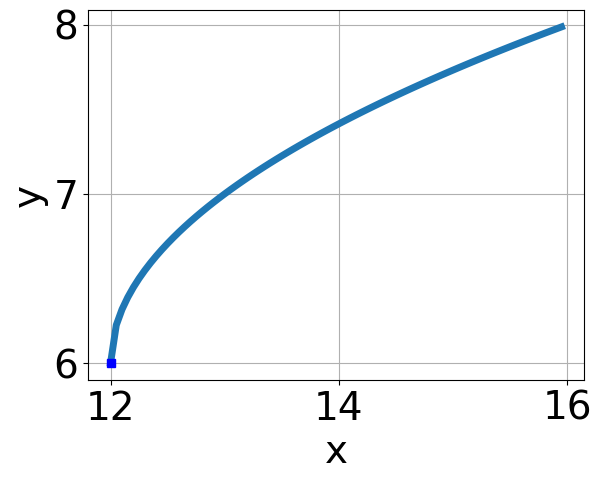
\includegraphics[width = 0.3\textwidth]{../Figures/radicalEquationToGraphCopyCC.png}\item 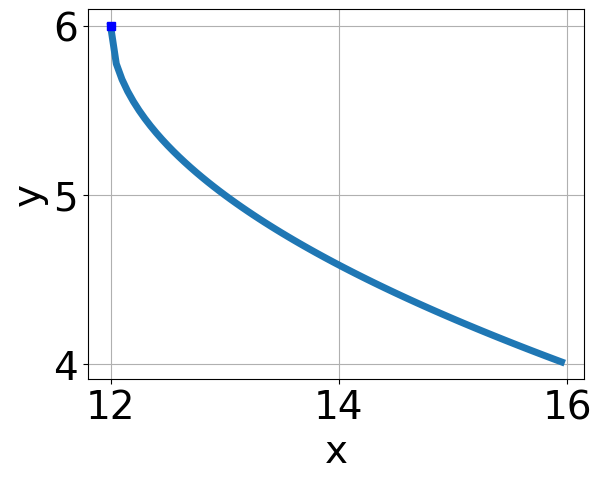
\includegraphics[width = 0.3\textwidth]{../Figures/radicalEquationToGraphCopyDC.png}\end{multicols}\item None of the above.
\end{enumerate} }
\litem{
What is the domain of the function below?\[ f(x) = \sqrt[8]{-8 x + 7} \]\begin{enumerate}[label=\Alph*.]
\item \( (-\infty, a], \text{ where } a \in [0.68, 1.07] \)
\item \( [a, \infty), \text{where } a \in [0.92, 1.43] \)
\item \( [a, \infty), \text{where } a \in [0.73, 0.91] \)
\item \( (-\infty, a], \text{where } a \in [0.99, 1.58] \)
\item \( (-\infty, \infty) \)

\end{enumerate} }
\end{enumerate}

\end{document}